\documentclass[twoside,a4paper]{article}
\usepackage{geometry}
\geometry{margin=1.5cm, vmargin={0pt,1cm}}
\setlength{\topmargin}{-1cm}
\setlength{\paperheight}{29.7cm}
\setlength{\textheight}{25.3cm}

% useful packages.
\usepackage{amsfonts}
\usepackage{amsmath}
\usepackage{amssymb}
\usepackage{amsthm}
\usepackage{enumerate}
\usepackage{graphicx}
\usepackage{multicol}
\usepackage{fancyhdr}
\usepackage{layout}
\usepackage{float}
\usepackage{mathtools}
% some common command
\newcommand{\dif}{\mathrm{d}}
\newcommand{\avg}[1]{\left\langle #1 \right\rangle}
\newcommand{\difFrac}[2]{\frac{\dif #1}{\dif #2}}
\newcommand{\pdfFrac}[2]{\frac{\partial #1}{\partial #2}}
\newcommand{\OFL}{\mathrm{OFL}}
\newcommand{\UFL}{\mathrm{UFL}}
\newcommand{\fl}{\mathrm{fl}}
\newcommand{\op}{\odot}
\newcommand{\Eabs}{E_{\mathrm{abs}}}
\newcommand{\Erel}{E_{\mathrm{rel}}}

\begin{document}

\pagestyle{fancy}
\fancyhead{}
\lhead{Jovi Wong(3180104829)}
\chead{Numerical Analysis homework \#8}
\rhead{2020/5/26}

\section*{I. Prove theorem 6.4 by assuming $\forall x \in (a,b)$ weight function $\rho(x)>0$}
\subsection*{a. prove $L_\rho^2[a,b]$ is a vector space}
$\forall u,v,w \in L_\rho^2[a,b]$ and $\forall a,b \in \mathbb{F}$ we can get following results easily
\begin{gather}
u+v=v+u\\
(u+v)+w=u+(v+w)\\
(ab)u=a(bu)\\
0+u=u\\
1u=u\\
(a+b)u=au+bv\\
a(u+v)=au+av
\end{gather}
where $0 \in L_\rho^2[a,b]$ and $1 \in \mathbb{F}$ . Besides, $\forall u$ , there exists $-u \in L_\rho^2[a,b]$ such that $u+v=0$, which satisfy all property of vector space. Hence proved. 
\subsection*{b. prove $L_\rho^2[a,b]$ is inner product space}
$\forall u,v,w \in L_\rho^2[a,b]$ and $\forall a \in \mathbb{F}$ assuming $\rho(x)>0$, we can get following results easily
\begin{gather}
<v,v>=\int_a^b \rho(x)v(x)\overline{v(x)} \dif x\geq 0\\
\end{gather}
Because $\rho(x)>0$ , $<v,v>=0$ iff $v(x)=0$ .
\begin{gather}
<u+v,w>=\int_a^b\rho(x)(u(x)+v(x))\overline{w(x)} \dif x = \int_a^b\rho(x)v(x)\overline{w(x)} \dif x + \int_a^b\rho(x)u(x)\overline{w(x)} \dif x = <u,w>+<v,w> \\
<av,w>=\int_a^ba\rho(x)v(x)\overline{w(x)} \dif x=a\int_a^b \rho(x)v(x)\overline{w(x)} \dif x = a<v,w>\\
<v,w>=\int_a^b \rho(x)v(x)\overline{w(x)} = \int_a^b \rho(x)\overline{\overline{v(x)}w(x)} \dif x = \overline{<w,v>}
\end{gather}
Hence $L_\rho^2[a,b]$ is an inner product space.

\section*{c. prove $L_\rho^2[a,b]$ is norm space}
From the definition of norm, we can know that $\forall v \in L_\rho^2[a,b]$
\begin{gather}
||v||_2=(\int_a^b \rho(x)|v(x)|^2 \dif x)^{\frac{1}{2}} =(\int_a^b \rho(x)v(x)\overline{v(x)} \dif x)^{\frac{1}{2}}=\sqrt{<v,v>}
\end{gather}
Hence proved.
\section*{II. Consider Chebyshev polynimials of the first kind}
\subsection*{a. Show that they are orthogonal on $[-1,1]$}
Because Chebyshev polinomials have form of $T_n(x)=\cos{(n\arccos{x})}$, we can deduce 
\begin{gather}
<T_n,T_m>=\int_a^b \frac{\cos{(n\arccos{x})}\cos{(m\arccos{x})}}{\sqrt{1-x^2}} \dif x
\end{gather}
Then we can take $x=\cos{\theta}$ into the above equation as following, where $\theta \in [0,\pi]$
\begin{gather}
<T_n,T_m>=-\int_0^\pi {\cos(m \theta) \cos{(n \theta)}}\dif \theta=-\int_0^\pi \frac{\cos{(m+n)\theta}+\cos{(m-n)\theta}}{2}=0
\end{gather}
Hence proved.
\subsection*{b. Normalize the first three Chebyshev polynomials}
The first three Chebyshev polynomials are as following 
\[ \left \{ \begin{lgathered}
u_1(x)=1 \\
u_2(x)=x \\
u_3(x)=2x^2-1
\end{lgathered} \right. \]
We can deduce as following steps. Firstly, 
\begin{gather}
v_1=u_1\\
u_1^*=\frac{v_1}{||v_1||}=\frac{1}{\sqrt{\pi}}
\end{gather}
Secondly,
\begin{gather}
v_2=u_2=x\\
u_2^*=\frac{v_2}{||v_2||}=\sqrt{\frac{2}{\pi}}x
\end{gather}
Thirdly,
\begin{gather}
v_3=u_3=2x^2-1\\
||v_3||=\sqrt{\int_{-1}^{1}\frac{(2x^2-1)^2}{\sqrt{1-x^2}} \dif x}=\sqrt{\int_{-\frac{\pi}{2}}^{\frac{\pi}{2}}(2\sin^2{\theta}-1)^2\dif \theta}=\sqrt{\frac{\pi}{2}}\\
u_3^*=\frac{v_3}{||v_3||}=\sqrt{\frac{2}{\pi}}(2x^2-1)
\end{gather}
\section*{III. Least-square approxiamation of a continuous function}
\subsection*{a. $\rho(x)=\frac{1}{\sqrt{1-x^2}}$ with Fourier expansion}
We select orthonormal polynomials in $\mathbb{P}_2$ as $u_1^*=\frac{1}{\sqrt{\pi}}$ , $u_2=\sqrt{\frac{2}{\pi}}x$ and $u_3=\sqrt{\frac{2}{\pi}}(2x^2-1)$ , then we can deduce that
\begin{gather}
<y,u_1^*>=\int_{-1}^1 \frac{1}{\sqrt{\pi}}2 \dif x = \frac{2}{\sqrt{\pi}} \\
<y,u_2^*>=\int_{-1}^1 \sqrt{\frac{2}{\pi}}x \dif x = 0 \\
<y,u_3^*>=\int_{-1}^1 \sqrt{\frac{2}{\pi}}(2x^2-1) \dif x= -\frac{2}{3}\sqrt{\frac{2}{\pi}}
\end{gather}
Therefore, the quadratic approxiamation of $y$ is $\varphi(x)=-\frac{8}{3\pi}x^2+\frac{10}{3\pi}$ .
\subsection*{b. $\rho(x)=\frac{1}{\sqrt{1-x^2}}$ with normal equation}
We select linearly independent a set of basis as $u_1=1$ , $u_2=x$ and $u_3=x^2$ , then
\[
G(u_1,u_2,u_3)= 
\begin{pmatrix}
\langle u_1,u_1 \rangle & \langle u_1,u_2 \rangle & \langle u_1,u_3 \rangle \\
\langle u_2,u_1 \rangle & \langle u_2,u_2 \rangle & \langle u_2,u_3 \rangle \\
\langle u_3,u_1 \rangle & \langle u_3,u_2 \rangle & \langle u_3,u_3 \rangle 
\end{pmatrix} =
\begin{pmatrix}
\pi & 0 & \frac{\pi}{2} \\
0 & \frac{\pi}{2} & 0 \\
\frac{\pi}{2} & 0 & \frac{3\pi}{8}
\end{pmatrix}
\]
\[
c =
\begin{pmatrix}
\langle y,u_1 \rangle & \langle y,u_2 \rangle & \langle y,u_3 \rangle 
\end{pmatrix}=
\begin{pmatrix}
2 & 0 & \frac{2}{3}
\end{pmatrix}
\]
As a result, we can get cofficents matrix by solving $Ga^T=c^T$ 
\[
a =
\begin{pmatrix}
\frac{10}{3\pi} & 0 & -\frac{8}{3\pi}
\end{pmatrix}
\]
Therefore, the quadratic approxiamation of $y$ is $\varphi(x)=-\frac{8}{3\pi}x^2+\frac{10}{3\pi}$ .

\section*{IV. Discrete least square via orthonormal polynomials}
\subsection*{a. Construct orthonormal polynomials by the Gram-Schmidt process}
The set of basis is as following 
\[ \left \{ \begin{lgathered}
u_1(x)=1 \\
u_2(x)=x \\
u_3(x)=x^2
\end{lgathered} \right. \]
We can deduce as following steps. Firstly, 
\begin{gather}
v_1=u_1=1\\
||v_1||= 2\sqrt{3} \approx 3.46\\
u_1^*=\frac{v_1}{||v_1||}=\frac{\sqrt{3}}{6} \approx 0.29
\end{gather}
Secondly,
\begin{gather}
v_2=u_2-<u_2,u_1^*>u_1^*=x-\frac{13}{2}\\
||v_2||=\sqrt{143} \approx 11.96 \\
u_2^*=\frac{v_2}{||v_2||}=\frac{x}{\sqrt{143}}-\frac{\sqrt{143}}{22} \approx \frac{x}{11.96}-0.54
\end{gather}
Thirdly,
\begin{gather}
v_3=u_3-\langle u_3,u_2^* \rangle u_2^*-\langle u_3,u_1^* \rangle u_1^* \approx x^2-13x+30.3\\
||v_3|| \approx  36.53\\
u_3^*=\frac{v_3}{||v_3||}=\frac{1}{36.53}x^2-\frac{13}{36.53}x+\frac{30.3}{36.53}
\end{gather}
\subsection*{b. Find the best approxiamation $\widehat{\varphi }=\sum_{i=0}^{2}a_ix^i$}
\[
G(u^*_1,u^*_2,u^*_3)= 
\begin{pmatrix}
\langle u^*_1,u^*_1 \rangle & \langle u^*_1,u^*_2 \rangle & \langle u^*_1,u^*_3 \rangle \\
\langle u^*_2,u^*_1 \rangle & \langle u^*_2,u^*_2 \rangle & \langle u^*_2,u^*_3 \rangle \\
\langle u_3^*,u_1^* \rangle & \langle u_3^*,u_2^* \rangle & \langle u_3^*,u_3^* \rangle 
\end{pmatrix} =
\begin{pmatrix}
1 & 0 & 0 \\
0 & 1 & 0 \\
0 & 0 & 1
\end{pmatrix}
\]
\[
c =
\begin{pmatrix}
\langle y,u^*_1 \rangle & \langle y,u^*_2 \rangle & \langle y,u^*_3 \rangle 
\end{pmatrix}=
\begin{pmatrix}
481.98 & 55.03 & 328.84
\end{pmatrix}
\]
Then the normal equation yield
\[
a = c=
\begin{pmatrix}
481.98 & 55.03 & 328.84
\end{pmatrix}
\]
Hence, 
\begin{gather}
\varphi(x)=328.84u_3^*+55.03u_2^*+481.98u_1^*=9.01x^2-112.42x+382.82
\end{gather}
which is very similar to the answer in the note.
\subsection*{c. Suppose there are other tables of sales. Which calculations can be reused?}
The orthonormal polynomials and Gram matrix can be reused. But we need to recalculate 
\[
c =
\begin{pmatrix}
\langle y,u^*_1 \rangle & \langle y,u^*_2 \rangle & \langle y,u^*_3 \rangle 
\end{pmatrix}
\]
The biggest advantage of orthonormal polynomials is that you can get the coefficents $a$ as soon as you can get matrix $c$ without solving equation $a=G^{-1}c$, because we have already known that $G^{-1}$ is an identity matrix.

\section*{Programming}
\begin{figure}[H]
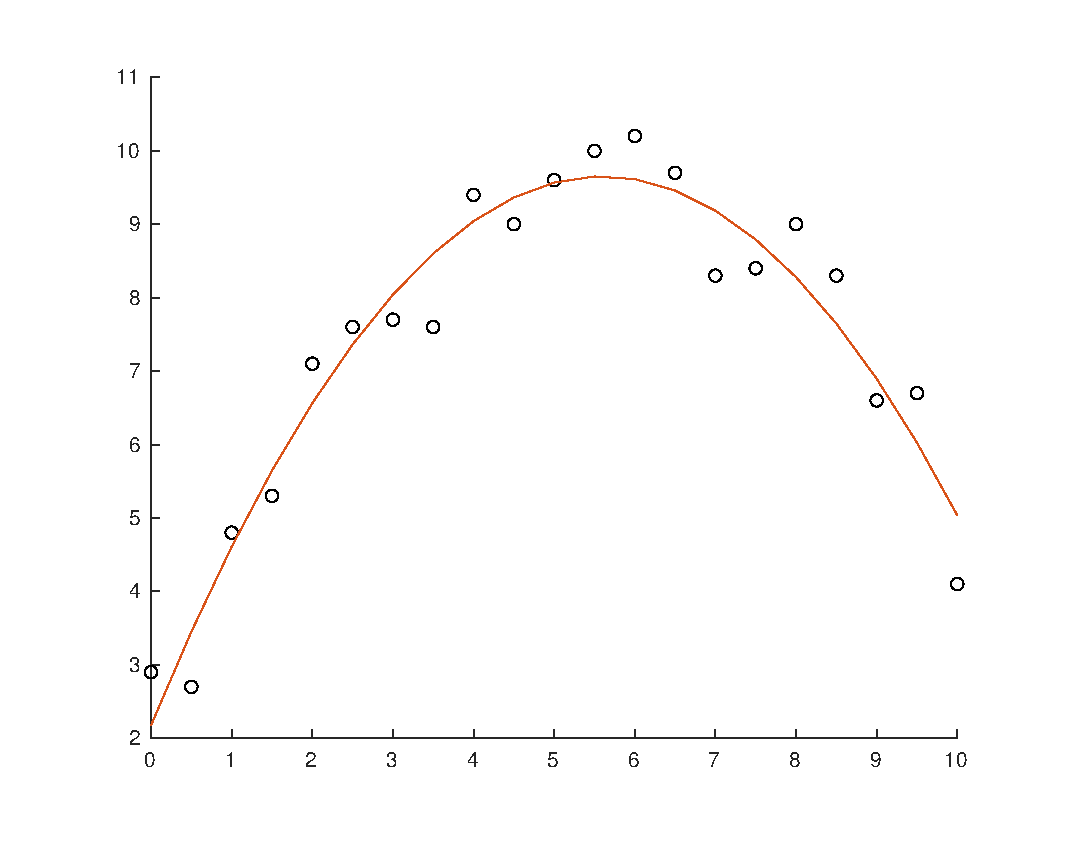
\includegraphics[width=7in]{DLS.eps}
\caption{Discrete Least Square via normal equations}
\end{figure}
The best approximation I find is $\varphi(x)=-0.238444*x^2+2.67041*x+2.17572$ .
\end{document}

%%% Local Variables: 
%%% mode: latex
%%% TeX-master: t
%%% End: 
